\documentclass[tikz,border=2pt]{standalone}
\usepackage{amsmath}
\usepackage{pgfplots}
\pgfplotsset{compat=1.18}
\usetikzlibrary{arrows.meta}
\begin{document}
% Purifying the chicken game. Top: with theta_i ~ U[-1,1] and epsilon = 0.1, types below the cutoff
% theta* = 0.3125 play S, types above play T, so T is played with probability (1 - theta*)/2 = 0.34375.
% Bottom: q(epsilon) = (1 + epsilon)/(3 + 2 epsilon) tends to the mixed-equilibrium value 1/3.
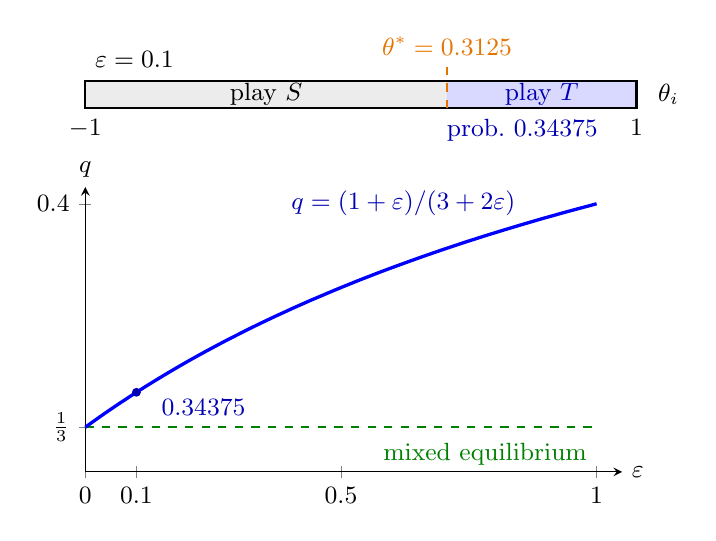
\begin{tikzpicture}[font=\small, >={Latex[length=2mm]}]
  % ---------- type line, x = 3.5 (theta + 1) cm ----------
  \fill[gray!15] (0,0) rectangle (4.594,0.35);
  \fill[blue!15] (4.594,0) rectangle (7,0.35);
  \draw[thick] (0,0) rectangle (7,0.35);
  \draw[orange!90!black, thick, dashed] (4.594,0) -- (4.594,0.55);
  \node at (2.297,0.175) {play $S$};
  \node[blue!70!black] at (5.797,0.175) {play $T$};
  \node[anchor=north] at (0,-0.02) {$-1$};
  \node[anchor=north] at (7,-0.02) {$1$};
  \node[orange!90!black, anchor=south] at (4.594,0.55) {$\theta^*=0.3125$};
  \node[anchor=west] at (7.15,0.175) {$\theta_i$};
  \node[blue!70!black, anchor=north] at (5.55,-0.02) {prob.\ $0.34375$};
  \node[anchor=south west] at (0,0.4) {$\varepsilon=0.1$};
  % ---------- limit as epsilon -> 0 ----------
  \begin{axis}[at={(0,-1.0cm)}, anchor=north west,
    width=8.4cm, height=5.2cm, axis lines=left,
    xmin=0, xmax=1.05, ymin=0.32, ymax=0.405,
    xtick={0,0.1,0.5,1}, ytick={0.3333333,0.4}, yticklabels={$\tfrac13$,$0.4$},
    xlabel={$\varepsilon$}, ylabel={$q$},
    xlabel style={anchor=west, at={(axis description cs:1,0)}},
    ylabel style={rotate=-90, anchor=south, at={(axis description cs:0,1)}},
    clip=false, every tick label/.append style={font=\small}]
    \addplot[green!50!black, thick, dashed, domain=0:1] {1/3};
    \addplot[blue, very thick, domain=0:1, samples=60] {(1+x)/(3+2*x)};
    \fill[blue!70!black] (axis cs:0.1,0.34375) circle (1.6pt);
    \node[blue!70!black, anchor=west] at (axis cs:0.13,0.3392) {$0.34375$};
    \node[blue!70!black, anchor=south east] at (axis cs:0.86,0.3935) {$q=(1+\varepsilon)/(3+2\varepsilon)$};
    \node[green!50!black, anchor=north east] at (axis cs:1.0,0.3315) {mixed equilibrium};
  \end{axis}
\end{tikzpicture}
\end{document}
